% The Dobbertin story, told in pictures.
% "Kasami Power Functions, Permutation Polynomials and Cyclic Difference Sets"
% Build with a Unicode engine (tectonic recommended):
%   tectonic dobbertin-story.tex
\documentclass[11pt]{article}

\usepackage[margin=1.05in]{geometry}
\usepackage{amsmath,amssymb}
\usepackage{xcolor}
\usepackage{fontspec}
\usepackage{listings}
\usepackage{tikz}
\usepackage{tikz-cd}
\usepackage[most]{tcolorbox}
\usepackage{colortbl}
\usetikzlibrary{positioning,arrows.meta,fit,backgrounds,calc,shapes.geometric,decorations.pathreplacing}

\usepackage{parskip}
\setlength{\parskip}{0.75em}
\linespread{1.08}

\newfontfamily\leanmono{DejaVu Sans Mono}[Scale=0.80]
\newfontfamily\dingfont{DejaVu Sans}

\newcommand{\ic}[1]{{\dingfont #1}}
\newcommand{\pencil}{\ic{✎}}
\newcommand{\bulb}{\ic{★}}
\newcommand{\spark}{\ic{✦}}
\newcommand{\hand}{\ic{☞}}
\newcommand{\gear}{\ic{✿}}

\definecolor{leanbg}{gray}{0.97}
\definecolor{leankw}{rgb}{0.30,0.20,0.65}
\definecolor{leancm}{rgb}{0.35,0.45,0.35}
\lstdefinestyle{lean}{
  backgroundcolor=\color{leanbg},
  basicstyle=\leanmono\small,
  keywordstyle=\color{leankw}\bfseries,
  commentstyle=\color{leancm}\itshape,
  morekeywords={def,theorem,lemma,structure,where,fun,Prop,Type,variable,
    namespace,end,open,noncomputable,Field,Fintype,Nat,import,Finset,
    Bijective,Function,by},
  morecomment=[l]{--},
  columns=fullflexible, keepspaces=true, showstringspaces=false,
  frame=single, framesep=6pt, xleftmargin=4pt,
  aboveskip=0.9em, belowskip=0.9em, extendedchars=true,
}
\lstset{style=lean}

% educational decoration boxes
\newtcolorbox{bigidea}{colback=blue!4,colframe=blue!55!black,
  fonttitle=\bfseries, title={\bulb\ \ BIG IDEA}, sharp corners=south,
  boxrule=0.7pt, left=6pt,right=6pt,top=4pt,bottom=4pt}
\newtcolorbox{remarkbox}{colback=gray!6,colframe=gray!60!black,
  fonttitle=\bfseries, title={\pencil\ \ IN THE PAPER}, sharp corners=south,
  boxrule=0.6pt, left=6pt,right=6pt,top=4pt,bottom=4pt}
\newtcolorbox{coolfact}{colback=orange!7,colframe=orange!70!black,
  fonttitle=\bfseries, title={\spark\ \ THE PATTERN}, sharp corners=south,
  boxrule=0.6pt, left=6pt,right=6pt,top=4pt,bottom=4pt}
\newtcolorbox{leanbox}{colback=green!5,colframe=green!45!black,
  fonttitle=\bfseries, title={\gear\ \ IN THE LEAN PROJECT}, sharp corners=south,
  boxrule=0.6pt, left=6pt,right=6pt,top=4pt,bottom=4pt}

% node styles reused across diagrams
\tikzset{
  thm/.style={draw,rounded corners,fill=blue!7,align=center,inner sep=4pt,font=\footnotesize},
  cor/.style={draw,rounded corners,fill=gray!8,align=center,inner sep=4pt,font=\footnotesize},
  conj/.style={draw,rounded corners,fill=orange!12,align=center,inner sep=4pt,font=\footnotesize},
  done/.style={draw,rounded corners,fill=green!12,align=center,inner sep=4pt,font=\footnotesize},
}

\title{\bf The Dobbertin Story, in Pictures\\[3pt]
  \large \emph{Kasami power functions, permutation polynomials, and cyclic difference sets}\\[2pt]
  \normalsize which structural patterns appear, and how they travel through the theorems}
\author{}
\date{}

\begin{document}
\maketitle

\begin{abstract}\noindent
One paper, six recurring \emph{shapes}. Each theorem, corollary, and the final
conjecture is one of these shapes wearing a new costume. This is a picture book:
little prose, many arrows. We name each pattern, draw it, point to where it lives
in Dobbertin (1999), and note how it is mirrored in the Lean project.
\end{abstract}

\begin{center}\small
$d = 2^{2k}-2^{k}+1$ \ (Kasami exponent), \quad $\gcd(k,n)=1$, \quad
$k'\equiv 1/k \pmod n$, \quad field $L=\mathrm{GF}(2^n)=\mathbb{F}_{2^n}$.
\end{center}

% =====================================================================
\section*{The whole paper on one page}
\addcontentsline{toc}{section}{The whole paper on one page}

\begin{center}
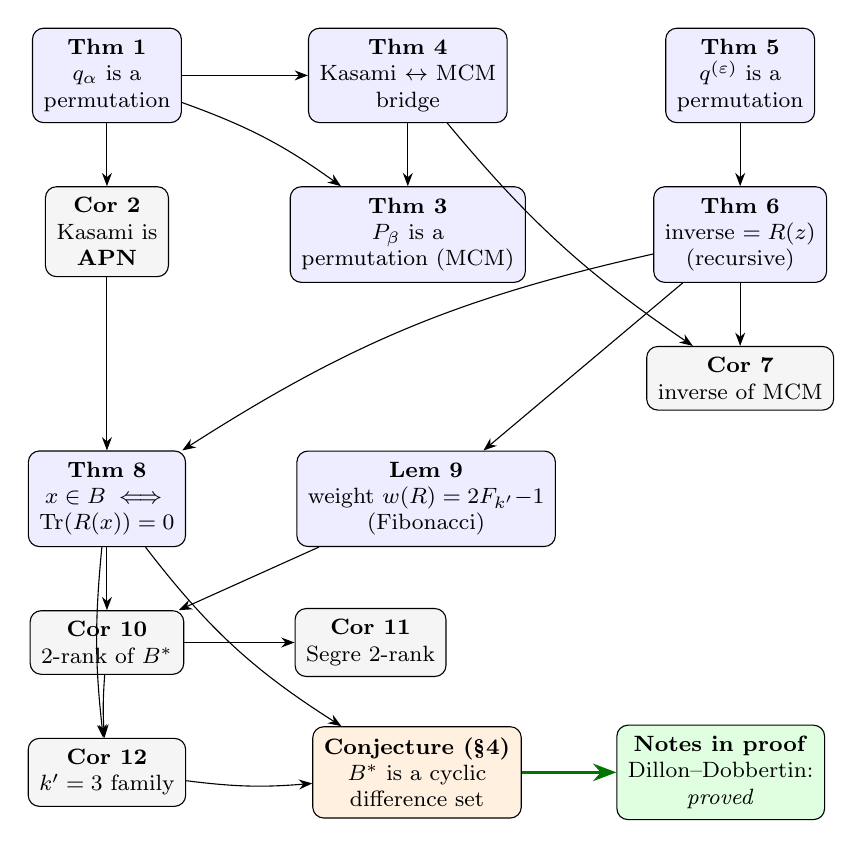
\begin{tikzpicture}[>=Stealth,node distance=6mm]
  % left column: permutation-polynomial spine
  \node[thm] (t1) {\textbf{Thm 1}\\ $q_\alpha$ is a\\ permutation};
  \node[cor,below=8mm of t1] (c2) {\textbf{Cor 2}\\ Kasami is\\ \textbf{APN}};
  \node[thm,right=16mm of t1] (t4) {\textbf{Thm 4}\\ Kasami $\leftrightarrow$ MCM\\ bridge};
  \node[thm,below=8mm of t4] (t3) {\textbf{Thm 3}\\ $P_\beta$ is a\\ permutation (MCM)};

  \node[thm,right=20mm of t4] (t5) {\textbf{Thm 5}\\ $q^{(\varepsilon)}$ is a\\ permutation};
  \node[thm,below=8mm of t5] (t6) {\textbf{Thm 6}\\ inverse $=R(z)$\\ (recursive)};
  \node[cor,below=8mm of t6] (c7) {\textbf{Cor 7}\\ inverse of MCM};

  \node[thm,below=22mm of c2] (t8) {\textbf{Thm 8}\\ $x\in B \iff$\\ $\mathrm{Tr}(R(x))=0$};
  \node[thm,right=14mm of t8] (l9) {\textbf{Lem 9}\\ weight $w(R)=2F_{k'}{-}1$\\ (Fibonacci)};
  \node[cor,below=8mm of t8] (c10) {\textbf{Cor 10}\\ 2-rank of $B^{*}$};
  \node[cor,right=14mm of c10] (c11) {\textbf{Cor 11}\\ Segre 2-rank};
  \node[cor,below=8mm of c10] (c12) {\textbf{Cor 12}\\ $k'=3$ family};

  \node[conj,right=16mm of c12] (cj) {\textbf{Conjecture ({\S}4)}\\ $B^{*}$ is a cyclic\\ difference set};
  \node[done,right=12mm of cj] (dn) {\textbf{Notes in proof}\\ Dillon--Dobbertin:\\ \emph{proved}};

  \draw[->] (t1)--(c2);
  \draw[->] (t1)--(t4);
  \draw[->] (t4)--(t3);
  \draw[->] (t1) to[bend left=8] (t3);
  \draw[->] (t5)--(t6);
  \draw[->] (t6)--(c7);
  \draw[->] (t4) to[bend right=8] (c7);
  \draw[->] (c2)--(t8);
  \draw[->] (t6) to[bend right=10] (t8);
  \draw[->] (t6)--(l9);
  \draw[->] (t8)--(c10);
  \draw[->] (l9)--(c10);
  \draw[->] (c10)--(c11);
  \draw[->] (t8) to[bend right=6] (c12);
  \draw[->] (c10) to[bend right=4] (c12);
  \draw[->] (t8) to[bend right=10] (cj);
  \draw[->] (c12) to[bend right=6] (cj);
  \draw[->,very thick,green!45!black] (cj)--(dn);
\end{tikzpicture}
\end{center}

\begin{center}\footnotesize
\textcolor{blue!55!black}{$\blacksquare$ theorem}\quad
\textcolor{gray!60!black}{$\blacksquare$ corollary}\quad
\textcolor{orange!80!black}{$\blacksquare$ conjecture}\quad
\textcolor{green!45!black}{$\blacksquare$ later proved}
\end{center}

\begin{bigidea}
Read left to right. \textbf{Permutations} give \textbf{APN}; the \textbf{bridge}
copies everything between two worlds; \textbf{inverting} a permutation gives an
explicit polynomial $R$; $R$ gives a \textbf{trace test} for a set $B$; the
\textbf{recursion} behind $R$ is \textbf{Fibonacci}, which fixes the \textbf{2-rank};
the trace test finally powers a \textbf{difference-set} conjecture.
\end{bigidea}

\newpage
% =====================================================================
\section*{The six patterns at a glance}
\addcontentsline{toc}{section}{The six patterns at a glance}

\begin{center}\small
\renewcommand{\arraystretch}{1.45}
\begin{tabular}{@{}c p{4.1cm} p{4.4cm} p{3.0cm}@{}}
\hline
\textbf{\#} & \textbf{pattern (simple English)} & \textbf{where in Dobbertin} & \textbf{Lean mirror}\\
\hline
P1 & \textbf{Two-to-one / width 2}: a map hits each value exactly $0$ or $2$ times & Cor 2 (APN); two-to-one map $t^{2^k}+t$ & \texttt{wid}, \texttt{WidthBdd}\\
P2 & \textbf{Bridge}: relabel by an invertible map, properties copy across & Thm 4 (Kasami $\leftrightarrow$ MCM), Thm 3 & \texttt{SiteEquiv}, \texttt{transport}\\
P3 & \textbf{Clock arithmetic}: exponents live on a circle of size $2^n{-}1$ & reduced normal form, cyclotomic cosets & \texttt{pow\_invariant\_mod}\\
P4 & \textbf{Fibonacci growth}: a two-step recursion counts the terms & Lem 9, $w(R)=2F_{k'}{-}1$; Cor 10/12 & recursion \& \texttt{Nat.fib}\\
P5 & \textbf{Quadratic echo}: whatever $2^k{+}1$ does, $2^{2k}{-}2^k{+}1$ echoes & Introduction; Cor 11; {\S}4 & Kasami vs.\ Gold\\
P6 & \textbf{Flat / ideal}: a count is perfectly even $\Rightarrow$ difference set & {\S}4 conjecture (ideal autocorrelation) & \texttt{WidthUnif}, flat spectrum\\
\hline
\end{tabular}
\end{center}

% =====================================================================
\section{P1 --- Two-to-one \ ($=$ width 2 \ $=$ APN)}

\textbf{Plain words:} the difference map lands on each target either $0$ times or exactly $2$ times.

\[
  x \;\longmapsto\; (x+a)^d + x^d \;=\; b
  \qquad\text{has \ }0\ \text{ or }\ 2\ \text{ solutions.}
\]

\begin{center}
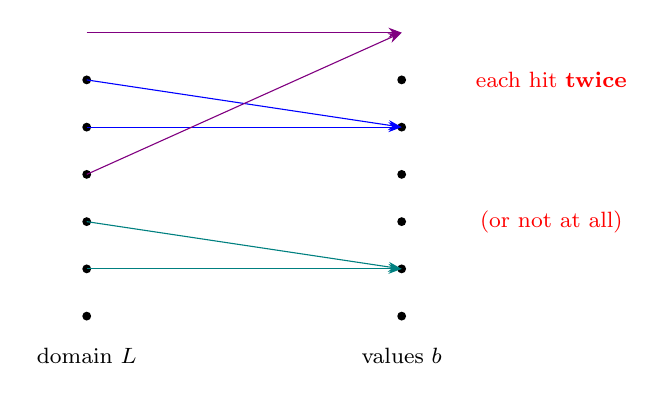
\begin{tikzpicture}[>=Stealth,every node/.style={font=\footnotesize}]
  % domain dots (left), codomain dots (right)
  \foreach \i in {0,...,5} \fill (0,\i*0.6) circle (1.6pt);
  \foreach \i in {0,...,5} \fill (4,\i*0.6) circle (1.6pt);
  \node at (0,-0.5) {domain $L$}; \node at (4,-0.5) {values $b$};
  % pair up: two arrows into same target
  \draw[->,blue] (0,3.0)--(4,2.4);
  \draw[->,blue] (0,2.4)--(4,2.4);
  \draw[->,teal] (0,1.2)--(4,0.6);
  \draw[->,teal] (0,0.6)--(4,0.6);
  \draw[->,violet] (0,3.6)--(4,3.6);
  \draw[->,violet] (0,1.8)--(4,3.6);
  \node[red] at (5.9,3.0) {each hit \textbf{twice}};
  \node[red] at (5.9,1.2) {(or not at all)};
\end{tikzpicture}
\end{center}

\begin{remarkbox}
Cor 2: ``Kasami power functions are almost perfect nonlinear.'' The engine is a
permutation $q$ (Thm 1) together with the two-to-one map $t\mapsto t^{2^k}+t$,
so $p(t)=\tfrac{1}{\Delta}\,q(t^{2^k}+t)$ is exactly $2$-to-$1$.
\end{remarkbox}

\begin{coolfact}
``$2$ solutions'' is the number that everything else is measured against:
\emph{width} $=$ size of a fibre. APN $=$ width $\le 2$.
\end{coolfact}

\begin{leanbox}
The project's \texttt{EWIGO} layer makes this the primitive object: the twisted
difference \texttt{tDiff}, its fibre \texttt{fib}, and the counter \texttt{wid}.
``APN'' is just \texttt{WidthBdd \_ 2}.
\begin{lstlisting}
def tDiff (d : ℕ) (a x : S.obj) : S.obj :=
  S.prod_ (S.endo d (S.prod_ x a)) (S.inv_ (S.endo d x))
def wid  (d : ℕ) (a b : S.obj) : ℕ := (fib S d a b).card
def WidthBdd (ω d : ℕ) : Prop :=
  ∀ a, a ≠ S.unit_ → ∀ b, wid S d a b ≤ ω
\end{lstlisting}
\end{leanbox}

% =====================================================================
\section{P2 --- The Bridge \ (transport along an invertible relabelling)}

\textbf{Plain words:} two families look different but a reversible dictionary
turns one into the other, so a proof on one side is free on the other.

\[
  \underbrace{q_\alpha}_{\text{Kasami}}
  \;\overset{\psi_\beta,\ \varphi_\alpha\;(\text{linear, invertible})}{\longleftrightarrow}\;
  \underbrace{P_\beta}_{\text{MCM}}
\]

\begin{center}
\begin{tikzcd}[column sep=2.3cm,row sep=1.1cm]
L \arrow[r,"q_\alpha"] \arrow[d,"\psi_\beta"',"\cong"] & L \\
L \arrow[r,"P_\beta"'] & L \arrow[u,"\varphi_\alpha"',"\cong"']
\end{tikzcd}
\qquad
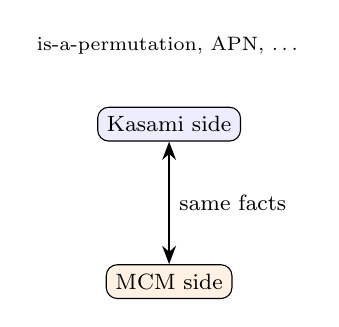
\begin{tikzpicture}[baseline=(current bounding box.center),>=Stealth,font=\footnotesize]
  \node[draw,rounded corners,fill=blue!7] (k) at (0,1) {Kasami side};
  \node[draw,rounded corners,fill=orange!10] (m) at (0,-1) {MCM side};
  \draw[<->,thick] (k)--(m) node[midway,right] {same facts};
  \node at (0,2.0) {\scriptsize is-a-permutation, APN, \dots};
\end{tikzpicture}
\end{center}

\begin{remarkbox}
Thm 4: an explicit \emph{linearized} substitution
$\psi_\beta(x)=\sum_{i<k}x^{2^i}+\beta\,\mathrm{Tr}(x)$ (and its inverse
$\varphi_\alpha$) gives a one-to-one correspondence
$q_\alpha\!\circ\!\psi_\beta = P_\beta$. Thm 3 (MCM is a permutation) then
falls out of Thm 1 for free. Dobbertin's own words: the Kasami polynomials are
``not new'' --- the bridge reveals they were MCM all along.
\end{remarkbox}

\begin{coolfact}
The dictionary is an \textbf{additive bijection} (a linearized polynomial). Any
property that only cares about the additive structure --- being a permutation,
being APN --- is \textbf{transported} unchanged.
\end{coolfact}

\begin{leanbox}
This is exactly the ``Caramello bridge'' formalised in
\texttt{Kasami/SiteEquivalences.lean}: \texttt{Pattern.transport} moves the
collision identity along a ring iso, \texttt{SiteEquiv} makes ``same picture''
an equivalence relation, and \texttt{width\_transport} proves the width count is
literally identical on both sides.
\end{leanbox}

% =====================================================================
\section{P3 --- Clock arithmetic on exponents \ (cyclotomic cosets)}

\textbf{Plain words:} for $x\ne0$ the exponent only matters modulo $2^n-1$, and
doubling an exponent (Frobenius $x\mapsto x^2$) just rotates its bit pattern.

\[
  x^{e} = x^{e \bmod (2^n-1)},
  \qquad
  e \sim 2e \sim 4e \sim \cdots \pmod{2^n-1}
  \ \ (\text{a cyclotomic coset}).
\]

\begin{center}
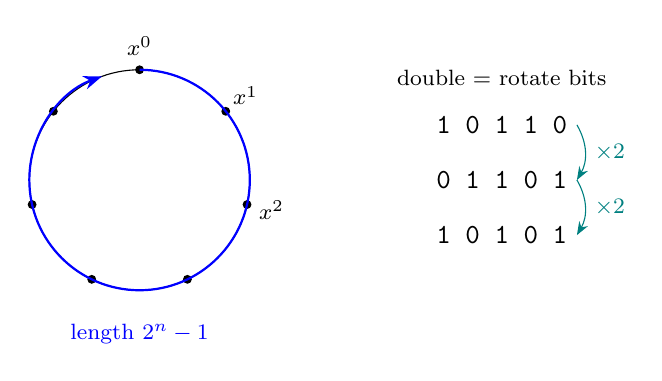
\begin{tikzpicture}[scale=1.0,>=Stealth,font=\footnotesize]
  \def\R{1.4}
  \draw (0,0) circle (\R);
  \foreach \i in {0,...,6}{\fill (90-\i*360/7:\R) circle (1.6pt);}
  \node at (90:\R+0.3){$x^{0}$};
  \node at (90-360/7:\R+0.32){$x^{1}$};
  \node at (90-2*360/7:\R+0.32){$x^{2}$};
  \draw[->,blue,thick] (90:\R) arc (90:-250:\R);
  \node[blue] at (0,-1.95){length $2^n-1$};
  % rotation of a bitstring
  \begin{scope}[xshift=4.6cm,yshift=0.2cm]
    \node at (0,1.1) {double $=$ rotate bits};
    \node[font=\ttfamily] (a) at (0,0.5) {1 0 1 1 0};
    \node[font=\ttfamily] (b) at (0,-0.2) {0 1 1 0 1};
    \node[font=\ttfamily] (c) at (0,-0.9) {1 0 1 0 1};
    \draw[->,teal] (a.east) to[bend left=30] node[right]{$\times2$} (b.east);
    \draw[->,teal] (b.east) to[bend left=30] node[right]{$\times2$} (c.east);
  \end{scope}
\end{tikzpicture}
\end{center}

\begin{remarkbox}
Used to build the \emph{reduced normal form} of $R$: reduce exponents mod
$2^n-1$, then cancel cyclotomic-equivalent powers (they give the same trace).
The whole rigidity argument in Lem 9 --- ``two exponents can't match by a
cyclic shift'' --- lives on this clock.
\end{remarkbox}

\begin{coolfact}
Frobenius $=$ ``rotate the bits''. Trace is blind to rotation. So the true
objects are \textbf{necklaces} of bits, not numbers.
\end{coolfact}

\begin{leanbox}
The atom \texttt{pow\_invariant\_mod} ($a\equiv b \Rightarrow x^a=x^b$ for
$x\ne0$) and the Frobenius bijection \texttt{frob\_bij} are the formal shadows of
this clock.
\end{leanbox}

% =====================================================================
\section{P4 --- Fibonacci growth \ (a two-step recursion counts terms)}

\textbf{Plain words:} the pieces of the inverse polynomial $R$ are built by
``new $=$ previous two'', so their term-counts are Fibonacci numbers.

\[
  A_{i+2} = (\cdots)A_{i+1} + (\cdots)A_i,
  \qquad
  w(A_i)=F_{i-1},\ \ w(B_i)=F_{i-2}
  \ \Longrightarrow\
  \boxed{\,w(R)=2F_{k'}-1\,}
\]

\begin{center}
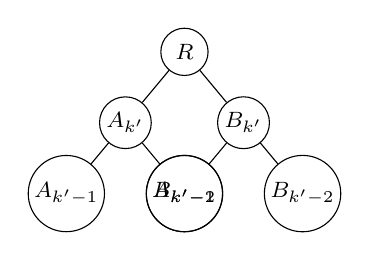
\begin{tikzpicture}[>=Stealth,font=\footnotesize,level distance=9mm,
   every node/.style={draw,circle,inner sep=1.2pt,minimum size=6mm}]
  \node {$R$}
    child {node {$A_{k'}$}
      child {node {$A_{k'-1}$}}
      child {node {$A_{k'-2}$}}}
    child {node {$B_{k'}$}
      child {node {$B_{k'-1}$}}
      child {node {$B_{k'-2}$}}};
\end{tikzpicture}
\qquad
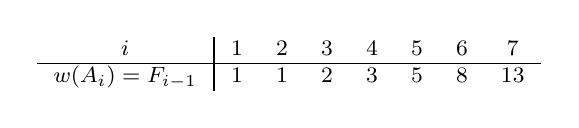
\begin{tikzpicture}[baseline=(current bounding box.center),font=\footnotesize]
  \node at (0,0) {\begin{tabular}{c|ccccccc}
    $i$ & 1 & 2 & 3 & 4 & 5 & 6 & 7\\\hline
    $w(A_i)=F_{i-1}$ & 1 & 1 & 2 & 3 & 5 & 8 & 13
  \end{tabular}};
\end{tikzpicture}
\end{center}

\begin{remarkbox}
Lem 9: $R$ is reduced iff $k'<n/2$, and $w(R)=2F_{k'}-1$ with
$F_0=F_1=1,\ F_{i+2}=F_{i+1}+F_i$. The Fibonacci count is exponential in $k'$
yet tiny compared to a random permutation polynomial --- that sparsity is the
whole point.
\end{remarkbox}

\begin{coolfact}
Count first, evaluate never. The 2-rank / linear span
$n(2F_{k_l}-1)+1$ (Cor 10) is \textbf{Fibonacci wearing a linear-algebra hat};
Cor 11 reads off the Segre 2-rank as the special case $k=2$.
\end{coolfact}

% =====================================================================
\section{P5 --- The Quadratic Echo \ ($2^k{+}1 \leadsto 2^{2k}{-}2^k{+}1$)}

\textbf{Plain words:} the easy quadratic exponent $2^k+1$ has nice properties;
the harder Kasami exponent $2^{2k}-2^k+1$ has the \emph{same} properties --- just
much harder to prove.

\begin{center}
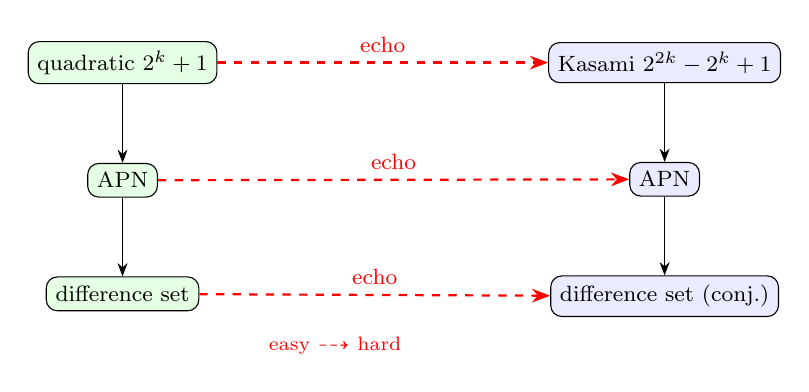
\begin{tikzpicture}[>=Stealth,font=\footnotesize,node distance=5mm]
  \node[draw,rounded corners,fill=green!10] (q1) {quadratic $2^k+1$};
  \node[draw,rounded corners,fill=green!10,below=10mm of q1] (q2) {APN};
  \node[draw,rounded corners,fill=green!10,below=10mm of q2] (q3) {difference set};
  \node[draw,rounded corners,fill=blue!8,right=42mm of q1] (k1) {Kasami $2^{2k}-2^k+1$};
  \node[draw,rounded corners,fill=blue!8,below=10mm of k1] (k2) {APN};
  \node[draw,rounded corners,fill=blue!8,below=10mm of k2] (k3) {difference set (conj.)};
  \draw[->] (q1)--(q2); \draw[->] (q2)--(q3);
  \draw[->] (k1)--(k2); \draw[->] (k2)--(k3);
  \draw[->,dashed,red,thick] (q1)-- node[above]{echo} (k1);
  \draw[->,dashed,red,thick] (q2)-- node[above]{echo} (k2);
  \draw[->,dashed,red,thick] (q3)-- node[above]{echo} (k3);
  \node[red] at (2.7,-3.6) {\scriptsize easy $\dashrightarrow$ hard};
\end{tikzpicture}
\end{center}

\begin{remarkbox}
Dobbertin, Introduction: ``It is an amazing observation that useful properties
of the quadratic exponent $2^k+1$ are often also shared by the Kasami exponent
$2^{2k}-2^k+1$ \dots\ but the known proofs for Kasami exponents require much more
effort.'' In {\S}4 he even conjectures these are (up to equivalence) the
\emph{only} exponents giving the difference-set property.
\end{remarkbox}

\begin{coolfact}
This meta-pattern is why the paper exists: transport the easy story to the hard
exponent. It is P2 (the bridge) applied to a whole \emph{theory}, not a single map.
\end{coolfact}

% =====================================================================
\section{P6 --- Flat / Ideal \ (perfectly even counts $\Rightarrow$ difference set)}

\textbf{Plain words:} if a shifted-correlation count is the \emph{same} for every
nonzero shift, the set is a (cyclic) difference set.

\[
  \sum_{x\in L} (-1)^{\,\mathrm{Tr}(R(x)+R(ax))} = 0
  \quad\text{for all } a\ne 1
  \;\;\Longleftrightarrow\;\;
  B^{*}\text{ is a difference set.}
\]

\begin{center}
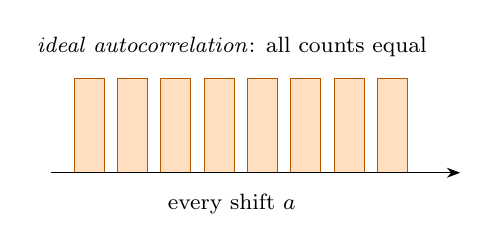
\begin{tikzpicture}[>=Stealth,font=\footnotesize]
  % flat bar chart: all bars equal height
  \foreach \i in {0,...,7} \filldraw[fill=orange!25,draw=orange!70!black]
     (\i*0.55,0) rectangle (\i*0.55+0.38,1.2);
  \node at (2.0,-0.4) {every shift $a$};
  \node at (2.0,1.6) {\emph{ideal autocorrelation}: all counts equal};
  \draw[->] (-0.3,0)--(4.9,0);
\end{tikzpicture}
\end{center}

\begin{remarkbox}
{\S}4 Conjecture: $B^{*}$ is a cyclic difference set with the \emph{Singer
parameters} $(2^n-1,\,2^{n-1}-1,\,2^{n-2}-1)$. Special cases already known:
$k=2$ gives Segre difference sets; $k'=2$ gives the Gong--Gaal--Golomb set;
$k'=3$ relates to the No--Chung--Yun conjecture. \textbf{Notes added in proof:}
proved by Dillon \& Dobbertin --- all listed conjectures confirmed.
\end{remarkbox}

\begin{coolfact}
``Flat'' is the second-moment twin of P1's ``width $2$''. A uniform width and a
flat spectrum are the same fact seen from two sides.
\end{coolfact}

\begin{leanbox}
The project records the uniform version as \texttt{WidthUnif} and proves the
second-moment identity \texttt{coll\_of\_uniform}
($\sum_b \mathtt{wid}^2 = \omega\cdot|S|$) --- the algebraic signature of
``flat''.
\begin{lstlisting}
def WidthUnif (ω d : ℕ) : Prop :=
  ∀ a, a ≠ S.unit_ → ∀ b, wid S d a b = 0 ∨ wid S d a b = ω
theorem coll_of_uniform (d ω : ℕ) (hω : 0 < ω) (hu : WidthUnif S ω d) ... :
    ∑ b, wid S d a b ^ 2 = ω * Fintype.card S.obj
\end{lstlisting}
\end{leanbox}

\newpage
% =====================================================================
\section*{How the patterns propagate}
\addcontentsline{toc}{section}{How the patterns propagate}

Each result is a \emph{combination} of the six shapes. Follow the coloured tags.

\begin{center}
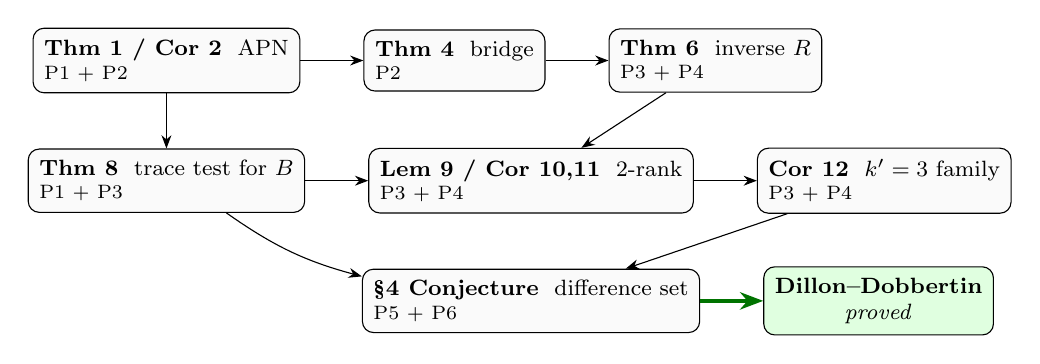
\begin{tikzpicture}[>=Stealth,font=\footnotesize,node distance=5mm,
   box/.style={draw,rounded corners,align=left,inner sep=4pt,fill=gray!4}]
  \node[box] (a) {\textbf{Thm 1 / Cor 2} \ APN\\[-1pt] \scriptsize P1 $+$ P2};
  \node[box,right=8mm of a] (b) {\textbf{Thm 4} \ bridge\\[-1pt] \scriptsize P2};
  \node[box,right=8mm of b] (c) {\textbf{Thm 6} \ inverse $R$\\[-1pt] \scriptsize P3 $+$ P4};
  \node[box,below=7mm of a] (d) {\textbf{Thm 8} \ trace test for $B$\\[-1pt] \scriptsize P1 $+$ P3};
  \node[box,right=8mm of d] (e) {\textbf{Lem 9 / Cor 10,11} \ 2-rank\\[-1pt] \scriptsize P3 $+$ P4};
  \node[box,right=8mm of e] (f) {\textbf{Cor 12} \ $k'=3$ family\\[-1pt] \scriptsize P3 $+$ P4};
  \node[box,below=7mm of e] (g) {\textbf{{\S}4 Conjecture} \ difference set\\[-1pt] \scriptsize P5 $+$ P6};
  \node[done,right=8mm of g] (h) {\textbf{Dillon--Dobbertin}\\ \emph{proved}};
  \draw[->] (a)--(b); \draw[->] (b)--(c);
  \draw[->] (a)--(d); \draw[->] (c)--(e); \draw[->] (d)--(e);
  \draw[->] (e)--(f);
  \draw[->] (d) to[bend right=10] (g);
  \draw[->] (f)--(g);
  \draw[->,very thick,green!45!black] (g)--(h);
\end{tikzpicture}
\end{center}

\begin{center}\small
\renewcommand{\arraystretch}{1.3}
\begin{tabular}{@{}l l@{}}
\hline
\textbf{step} & \textbf{patterns fired}\\
\hline
Kasami is a permutation, hence APN & P1 (two-to-one) $+$ P2 (bridge to MCM)\\
Explicit inverse $R$ & P3 (clock) $+$ P4 (Fibonacci recursion)\\
$x\in B \iff \mathrm{Tr}(R(x))=0$ & P1 (fibres) $+$ P3 (trace / cosets)\\
2-rank and Segre / $k'=3$ families & P3 (necklaces) $+$ P4 (Fibonacci)\\
$B^{*}$ is a cyclic difference set & P5 (quadratic echo) $+$ P6 (flat/ideal)\\
\hline
\end{tabular}
\end{center}

\begin{bigidea}
The paper is a \emph{relay race}. P1 starts it (count fibres); P2 duplicates the
lane (Kasami $\equiv$ MCM); P3+P4 build an explicit, sparse inverse; that inverse
turns the geometric set $B$ into a trace test; and P5+P6 hand the baton to a
difference-set conjecture --- later crossed the finish line by Dillon \& Dobbertin.
\end{bigidea}

% =====================================================================
\section*{Where the patterns live in the Lean project}
\addcontentsline{toc}{section}{Where the patterns live in the Lean project}

\begin{center}\small
\renewcommand{\arraystretch}{1.35}
\begin{tabular}{@{}c p{5.2cm} p{6.0cm}@{}}
\hline
\textbf{pattern} & \textbf{Dobbertin object} & \textbf{Lean declaration / file}\\
\hline
P1 & two-to-one map; APN; width $2$ & \texttt{tDiff}, \texttt{fib}, \texttt{wid}, \texttt{WidthBdd} \ (\texttt{EWIGO})\\
P2 & Thm 4 Kasami $\leftrightarrow$ MCM & \texttt{SiteEquiv}, \texttt{Pattern.transport}, \texttt{width\_transport} \ (\texttt{Kasami/SiteEquivalences.lean})\\
P3 & cyclotomic cosets, reduced form & \texttt{pow\_invariant\_mod}, \texttt{frob\_bij} \ (\texttt{Kasami/InvariantPatterns.lean})\\
P4 & recursions $A_i,B_i,C_i$; $w(R)$ & Fibonacci counting, \texttt{Nat.fib}\\
P5 & quadratic vs.\ Kasami exponent & Gold vs.\ Kasami power maps\\
P6 & ideal autocorrelation, difference set & \texttt{WidthUnif}, \texttt{coll\_of\_uniform}; flat-spectrum reading\\
\hline
\end{tabular}
\end{center}

\begin{center}
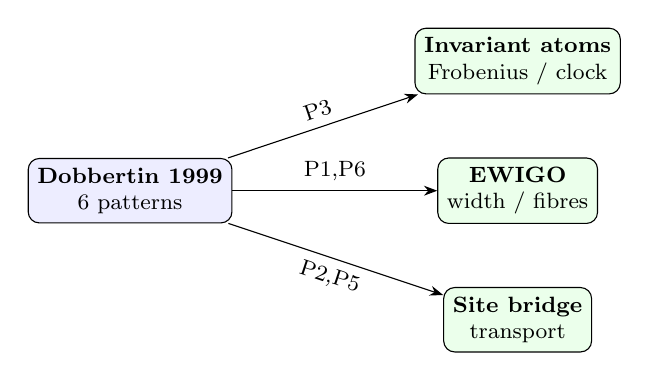
\begin{tikzpicture}[>=Stealth,font=\footnotesize,node distance=4mm,
   every node/.style={align=center}]
  \node[draw,rounded corners,fill=blue!7] (paper) {\textbf{Dobbertin 1999}\\ 6 patterns};
  \node[draw,rounded corners,fill=green!8,right=26mm of paper] (ewigo) {\textbf{EWIGO}\\ width / fibres};
  \node[draw,rounded corners,fill=green!8,below=8mm of ewigo] (bridge) {\textbf{Site bridge}\\ transport};
  \node[draw,rounded corners,fill=green!8,above=8mm of ewigo] (inv) {\textbf{Invariant atoms}\\ Frobenius / clock};
  \draw[->] (paper) to node[above,sloped]{P1,P6} (ewigo);
  \draw[->] (paper) to node[below,sloped]{P2,P5} (bridge);
  \draw[->] (paper) to node[above,sloped]{P3} (inv);
\end{tikzpicture}
\end{center}

% =====================================================================
\section*{One sentence to remember}
\addcontentsline{toc}{section}{One sentence to remember}

\begin{center}\large
\hand\ \ \emph{Count fibres (P1), copy across a bridge (P2), work on the exponent
clock (P3), let Fibonacci do the counting (P4), echo the quadratic case (P5),
and check for flatness (P6) --- that is the whole Dobbertin paper.}
\end{center}

\end{document}
